\section{Additional Results of Sample Size Experiment}\label{sec:additional-results}

Figures \ref{fig:eye-sample-size-results-results-02} and \ref{fig:eye-sample-size-results-results-03} display the results of re-running the sample size experiment from Section \ref{sec:sample-size-experiment} with a different value of the random seed.
There are differences due to the variability induced in the sub-sampling, but the general patterns identified in Section \ref{sec:sample-size-experiment} remain the same.

\begin{figure}
    \centering
    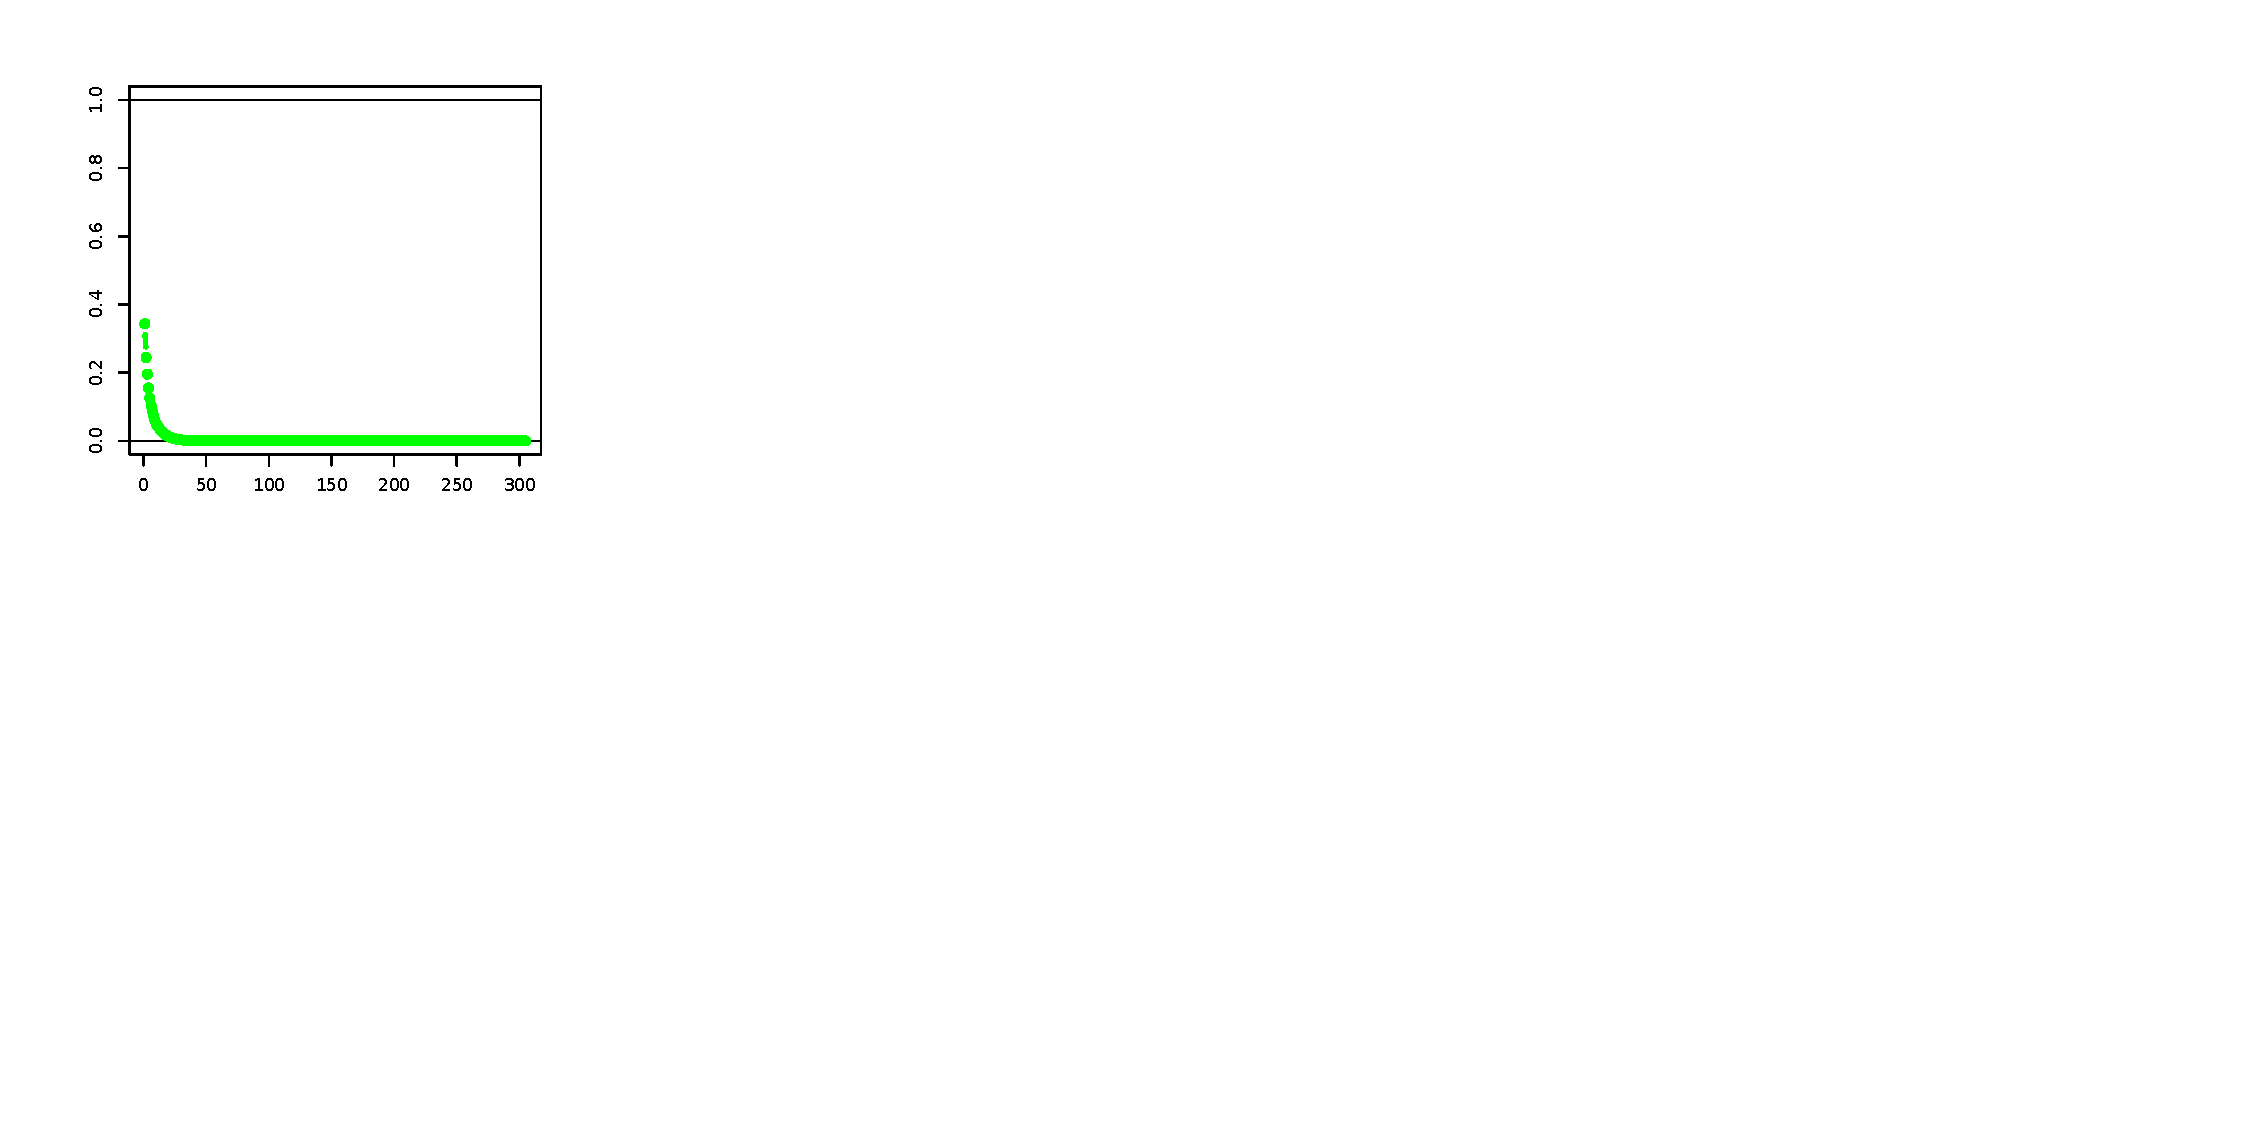
\includegraphics[width=1\linewidth]{figures/eye-sample-size-results-results-real-02.pdf}
    \caption{Results of re-running the sample size experiment presented in Figure \ref{fig:eye-sample-size-results-results-01} with a different random seed.}
    \label{fig:eye-sample-size-results-results-02}
\end{figure}

\begin{figure}
    \centering
    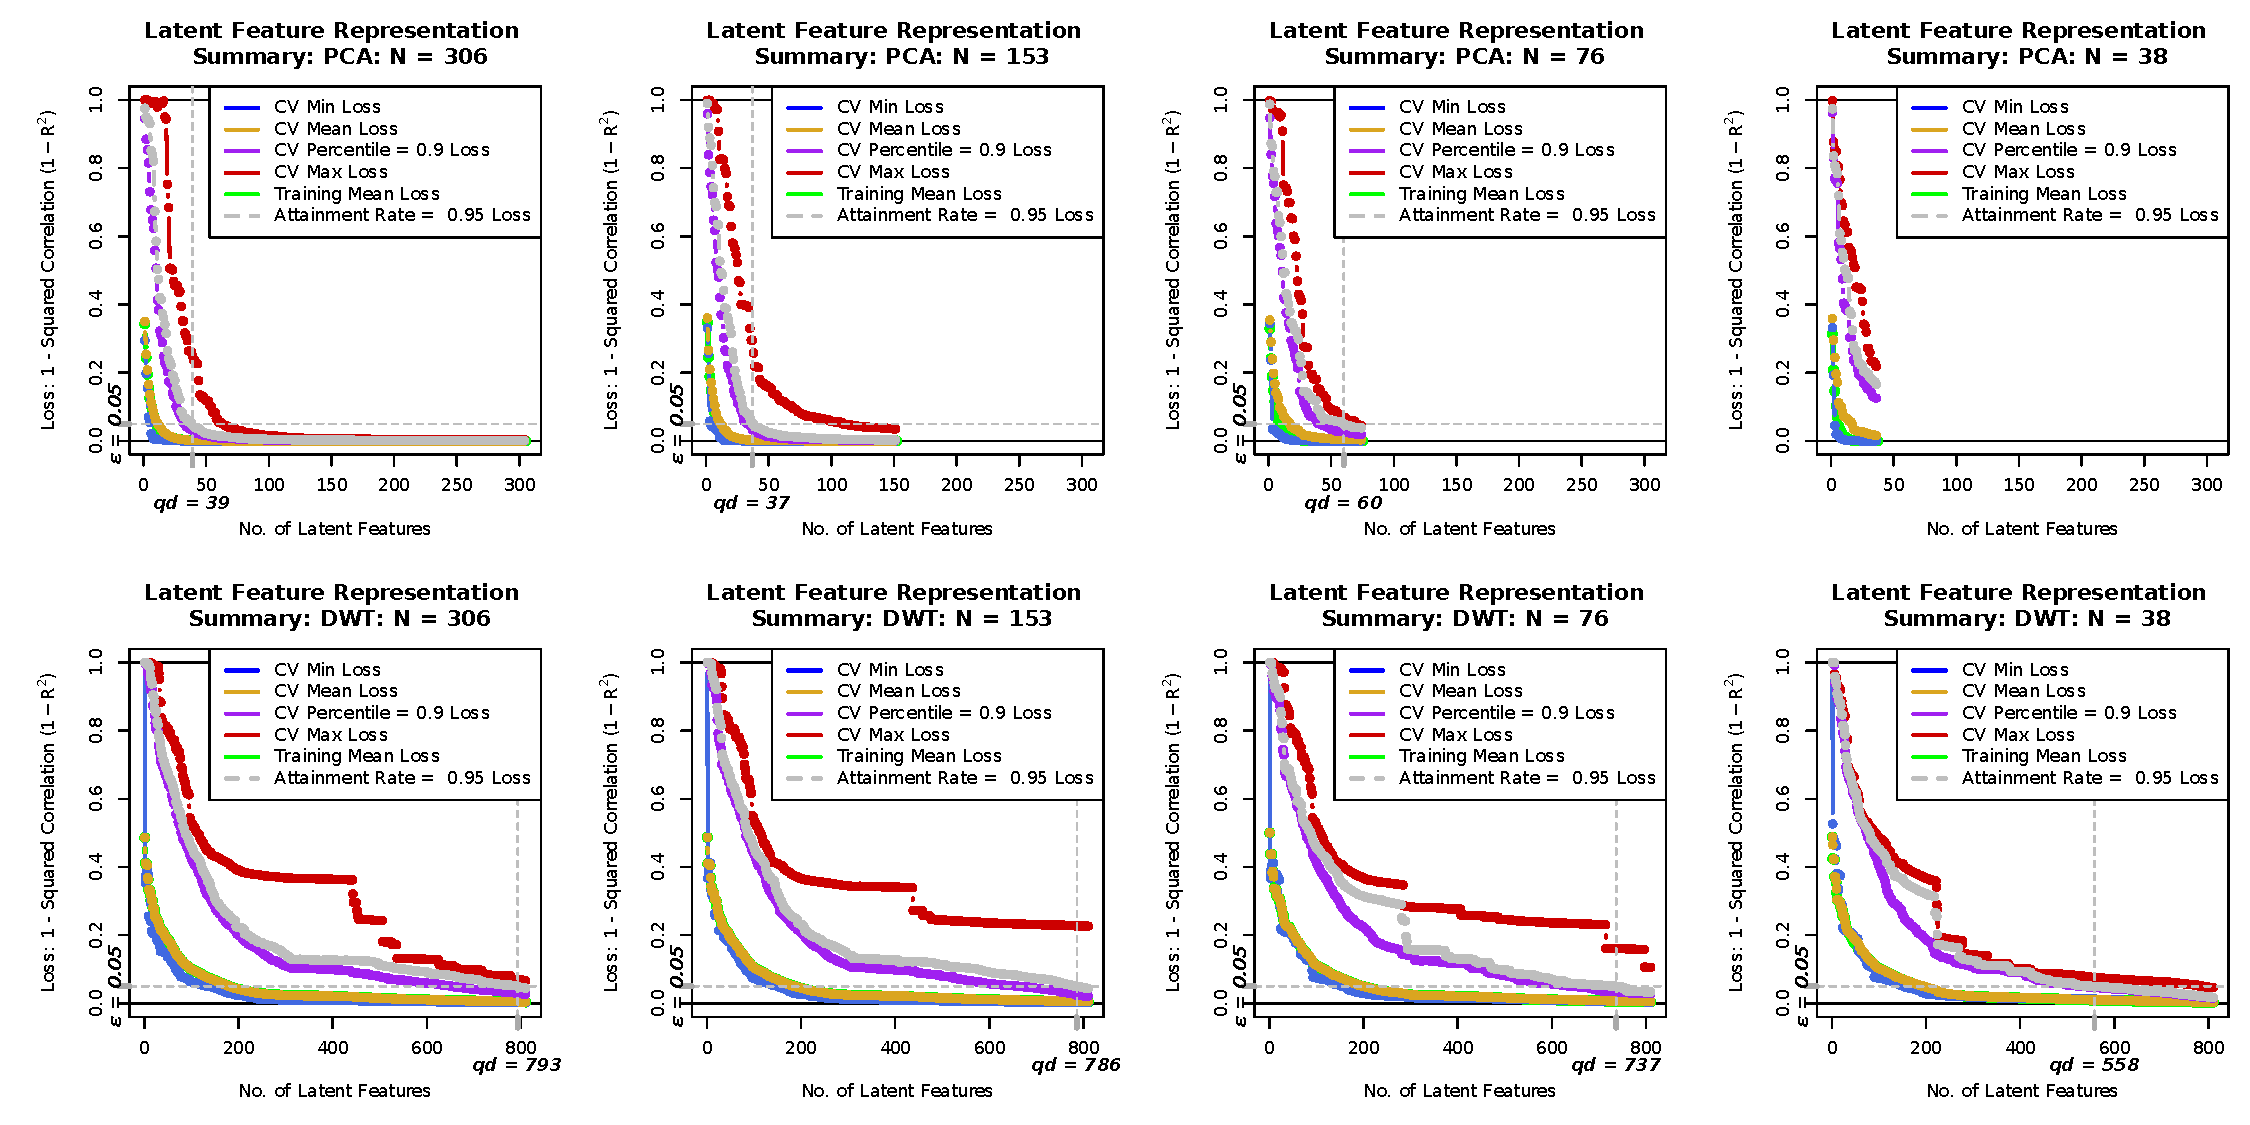
\includegraphics[width=1\linewidth]{figures/eye-sample-size-results-results-real-03.pdf}
    \caption{Results of re-running the sample size experiment presented in Figure \ref{fig:eye-sample-size-results-results-01} with a different random seed.}
    \label{fig:eye-sample-size-results-results-03}
\end{figure}